\subsection{Lab2: Osciloscopio y FFT}
%*********************
\begin{frame}{}

\pgfdeclareimage[width=\paperwidth,height=\paperheight]{bg}{imagenes/fondo_lab}
\setbeamertemplate{background}{\pgfuseimage{bg}}

\bfseries{\textrm{\LARGE Lab2\\ \Large Osciloscopio y FFT}}
\raggedright
\end{frame}
%*********************

%-----------------------------------
\begin{frame}{Osciloscopio y FFT\index{TCP}}

\pgfdeclareimage[width=\paperwidth,height=\paperheight]{bg}{imagenes/fondo3}
\setbeamertemplate{background}{\pgfuseimage{bg}}

En este laboratorio se genera una onda senoidal y a su vez algún ruido; estas dos señales se suman y se observa el resultado en el dominio de la frecuencia (FFT) y del tiempo (Scope). Se aprende a utilizar el notebook y algunas herramientas básicas del GRC. 

\end{frame}
%---------------------------------

\begin{frame}{Osciloscopio y FFT\index{TCP}}

\begin{figure}[H]
\vspace{-4mm}
\centering
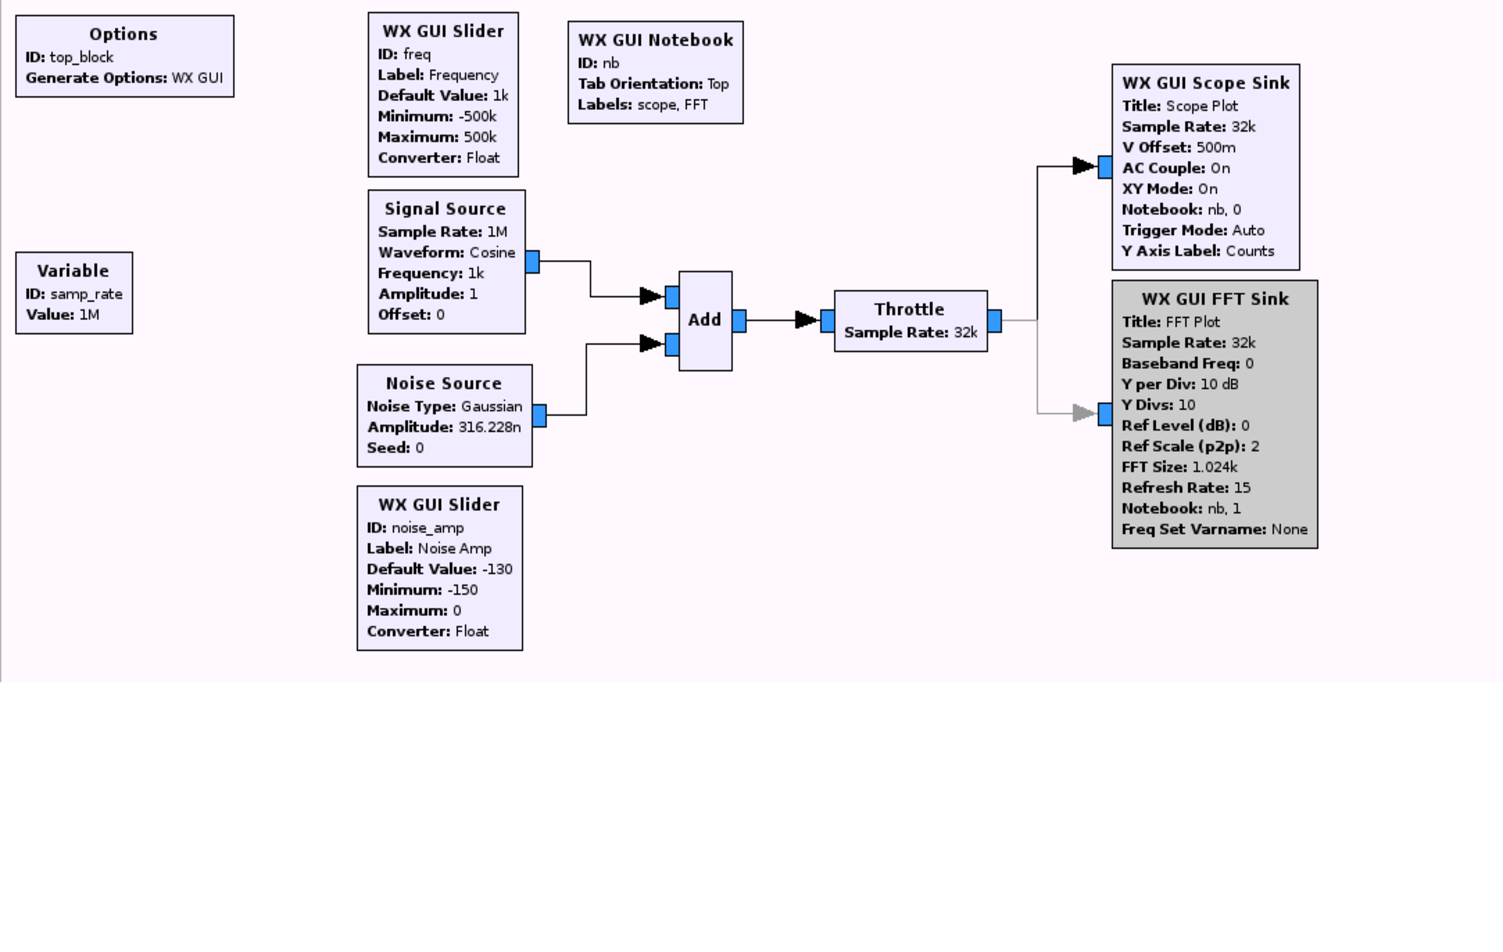
\includegraphics[width=1.2\textwidth]{parte1/lab2/pdf/lab2_1.pdf}
\end{figure}
\end{frame}
%---------------------------------

\begin{frame}{Osciloscopio y FFT}
\begin{figure}[H]
\vspace{-4mm}
\centering
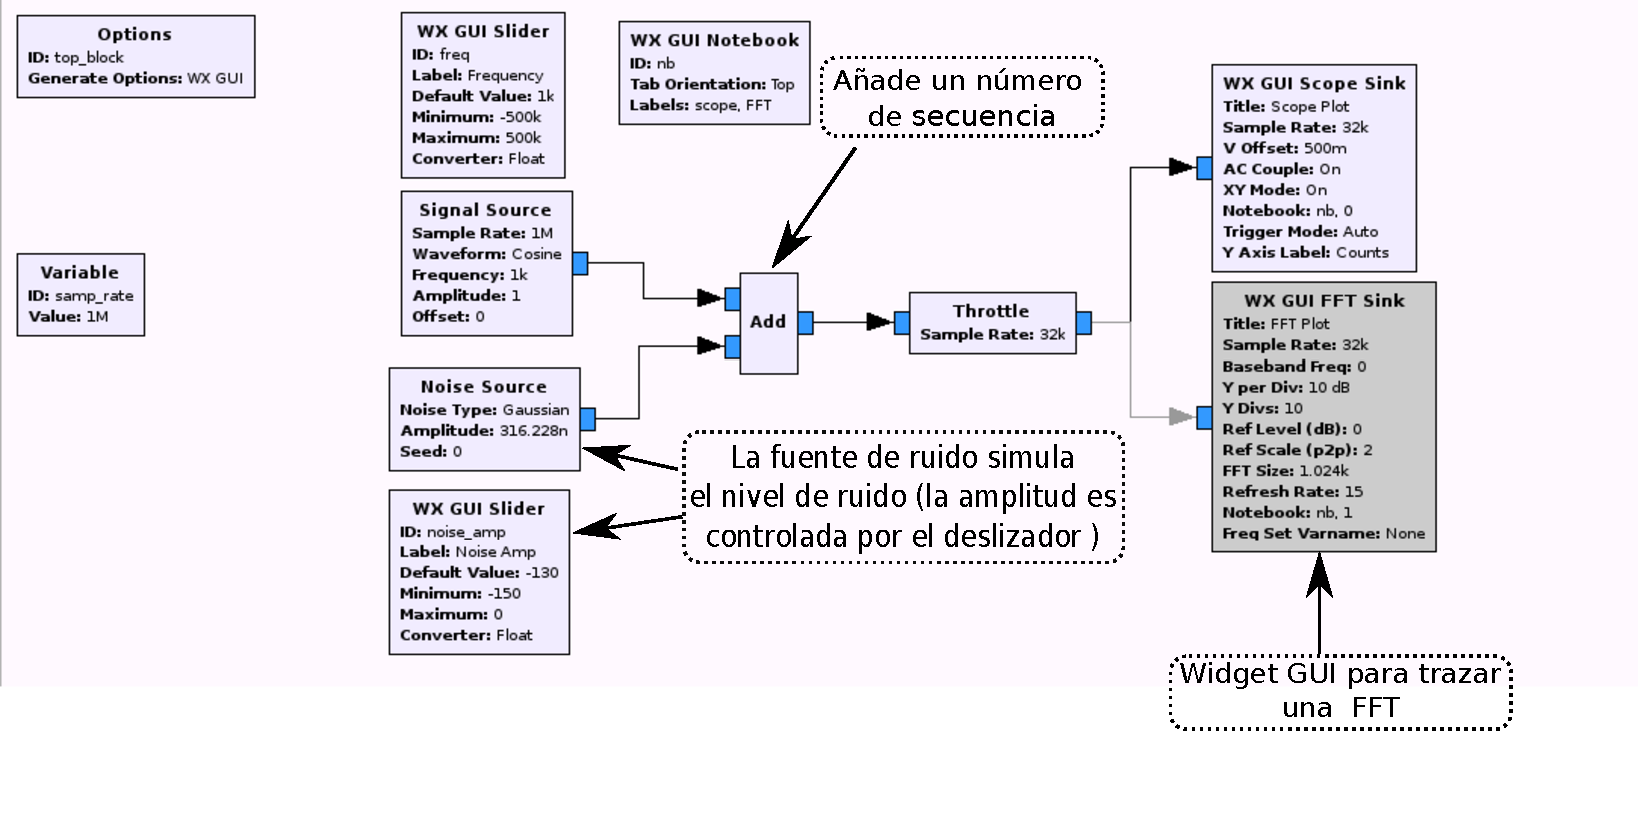
\includegraphics[width=1.1\textwidth]{parte1/lab2/pdf/lab2_2.pdf}
\end{figure}
\end{frame}
%--------------------------------

\begin{frame}{Osciloscopio y FFT\index{Noise Source}}
\begin{figure}[H]
\centering
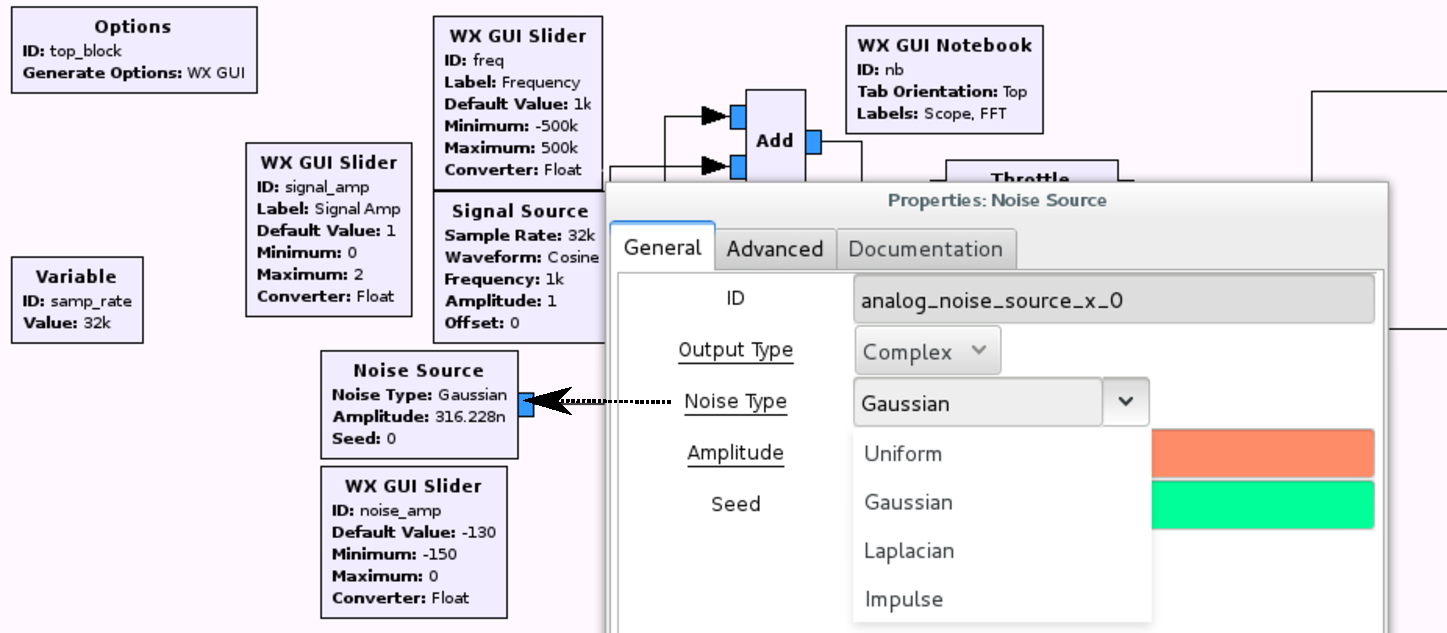
\includegraphics[width=1.055\textwidth]{parte1/lab2/pdf/lab2_3.pdf}
\end{figure}
\end{frame}
%--------------------------------

\begin{frame}{Osciloscopio y FFT\index{Noise Source}}
\begin{figure}[H]
\centering
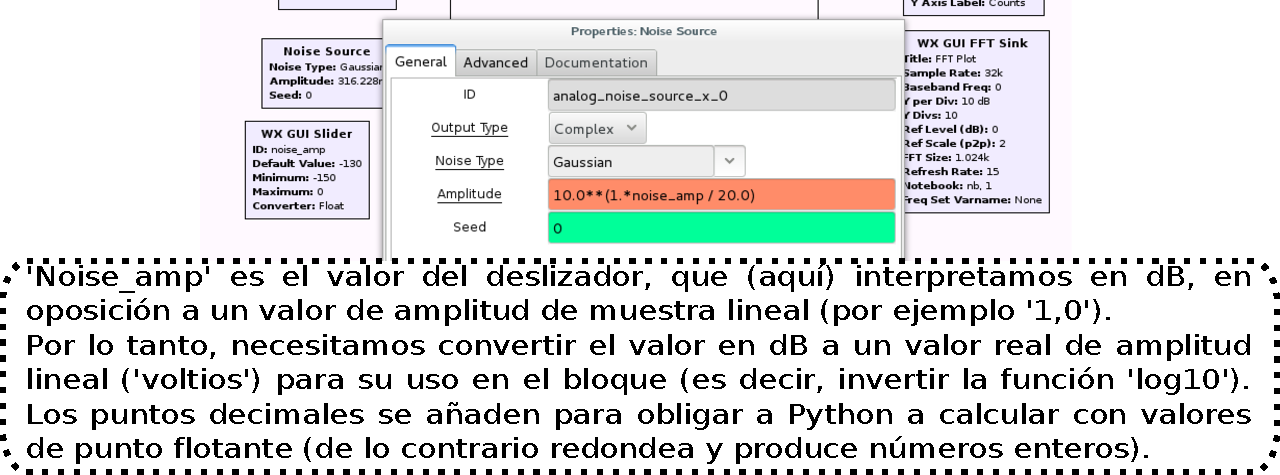
\includegraphics[width=1.055\textwidth]{parte1/lab2/pdf/lab2_4.pdf}
\end{figure}
\end{frame}
%--------------------------------

\begin{frame}{Osciloscopio y FFT\index{Add}}
\begin{figure}[H]
\centering
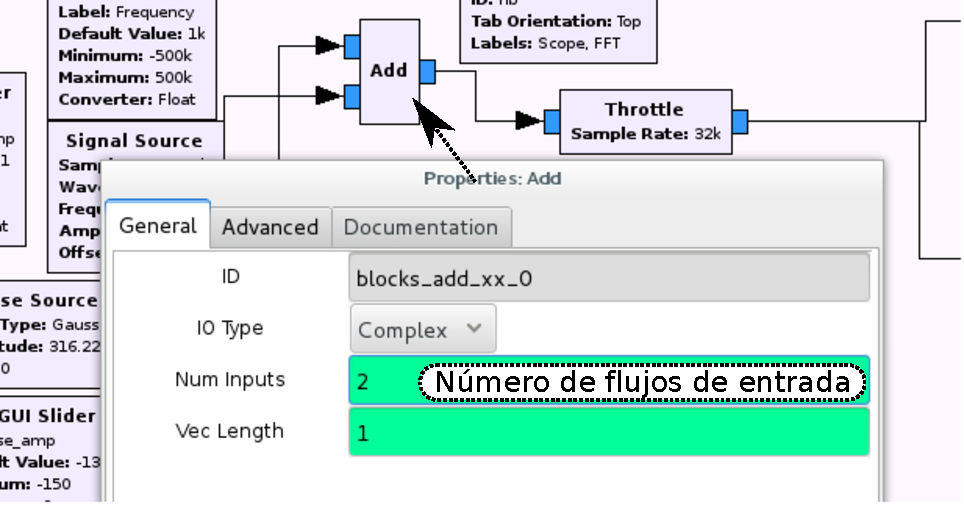
\includegraphics[width=.7\textwidth]{parte1/lab2/pdf/lab2_5.pdf}
\end{figure}
\end{frame}
%--------------------------------

\begin{frame}{Osciloscopio y FFT}
\begin{figure}[H]
\vspace{-4mm}
\centering
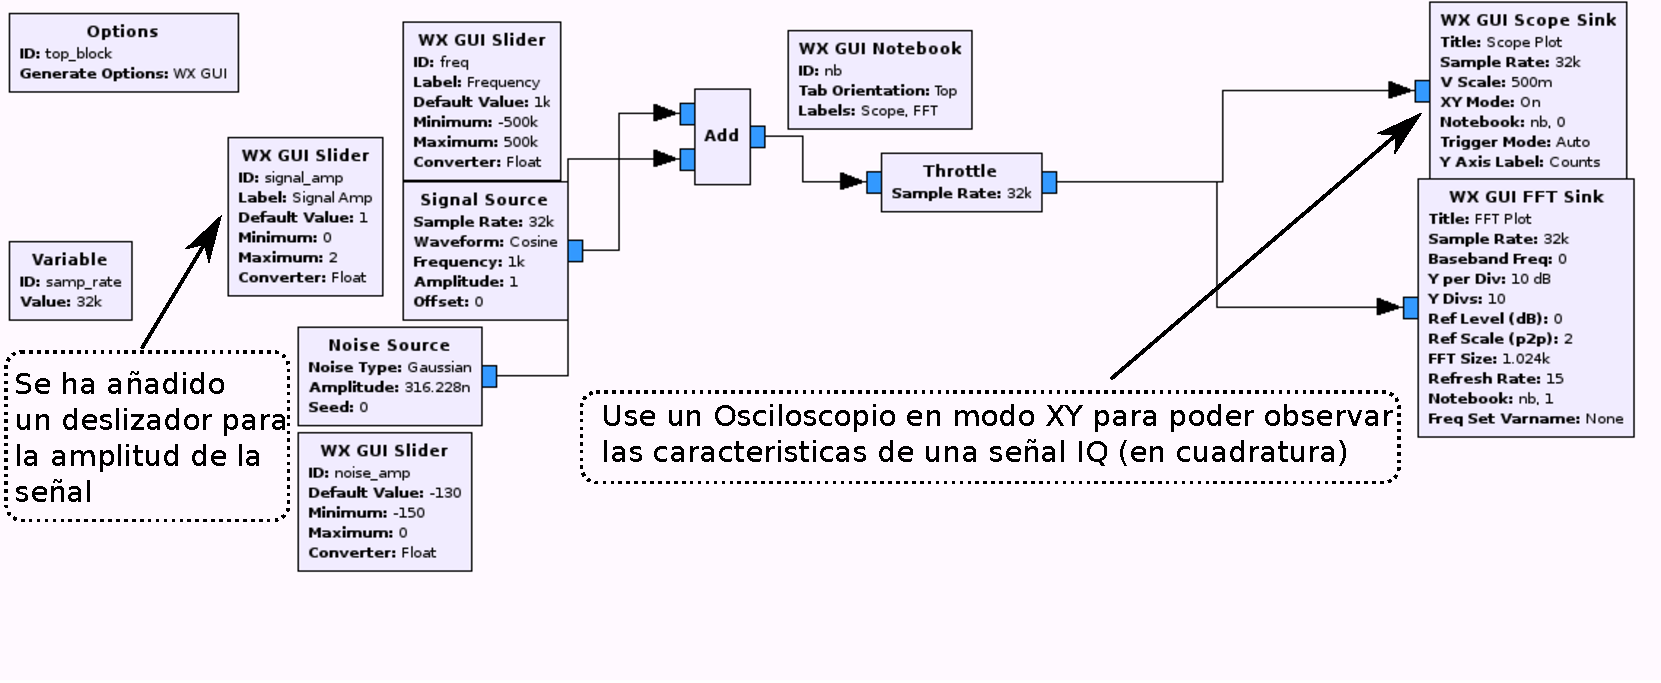
\includegraphics[width=1.1\textwidth]{parte1/lab2/pdf/lab2_6.pdf}
\end{figure}
\end{frame}
%--------------------------------

\begin{frame}{Osciloscopio y FFT\index{WX GUI Notebook}}
\begin{figure}[H]
\vspace{-4mm}
\centering
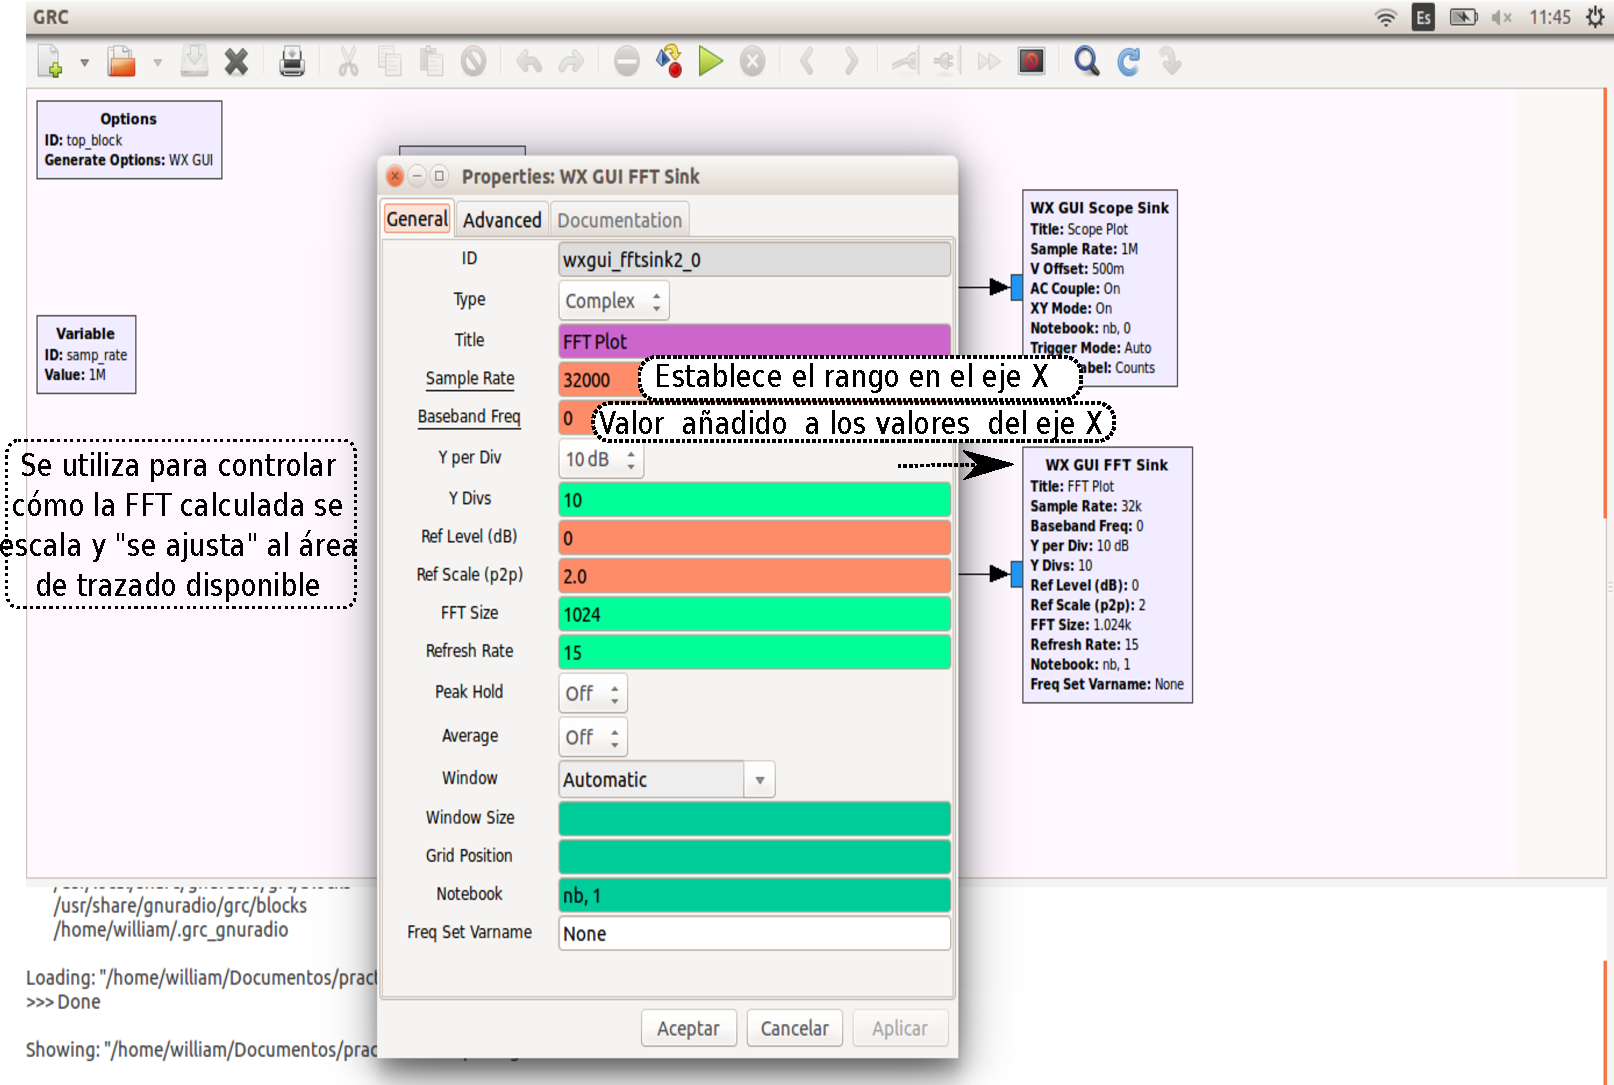
\includegraphics[width=0.85\textwidth]{parte1/lab2/pdf/lab2_7.pdf}
\end{figure}
\end{frame}
%--------------------------------

\begin{frame}{Osciloscopio y FFT\index{WX GUI FFT Sink}}
\begin{figure}[H]
\centering
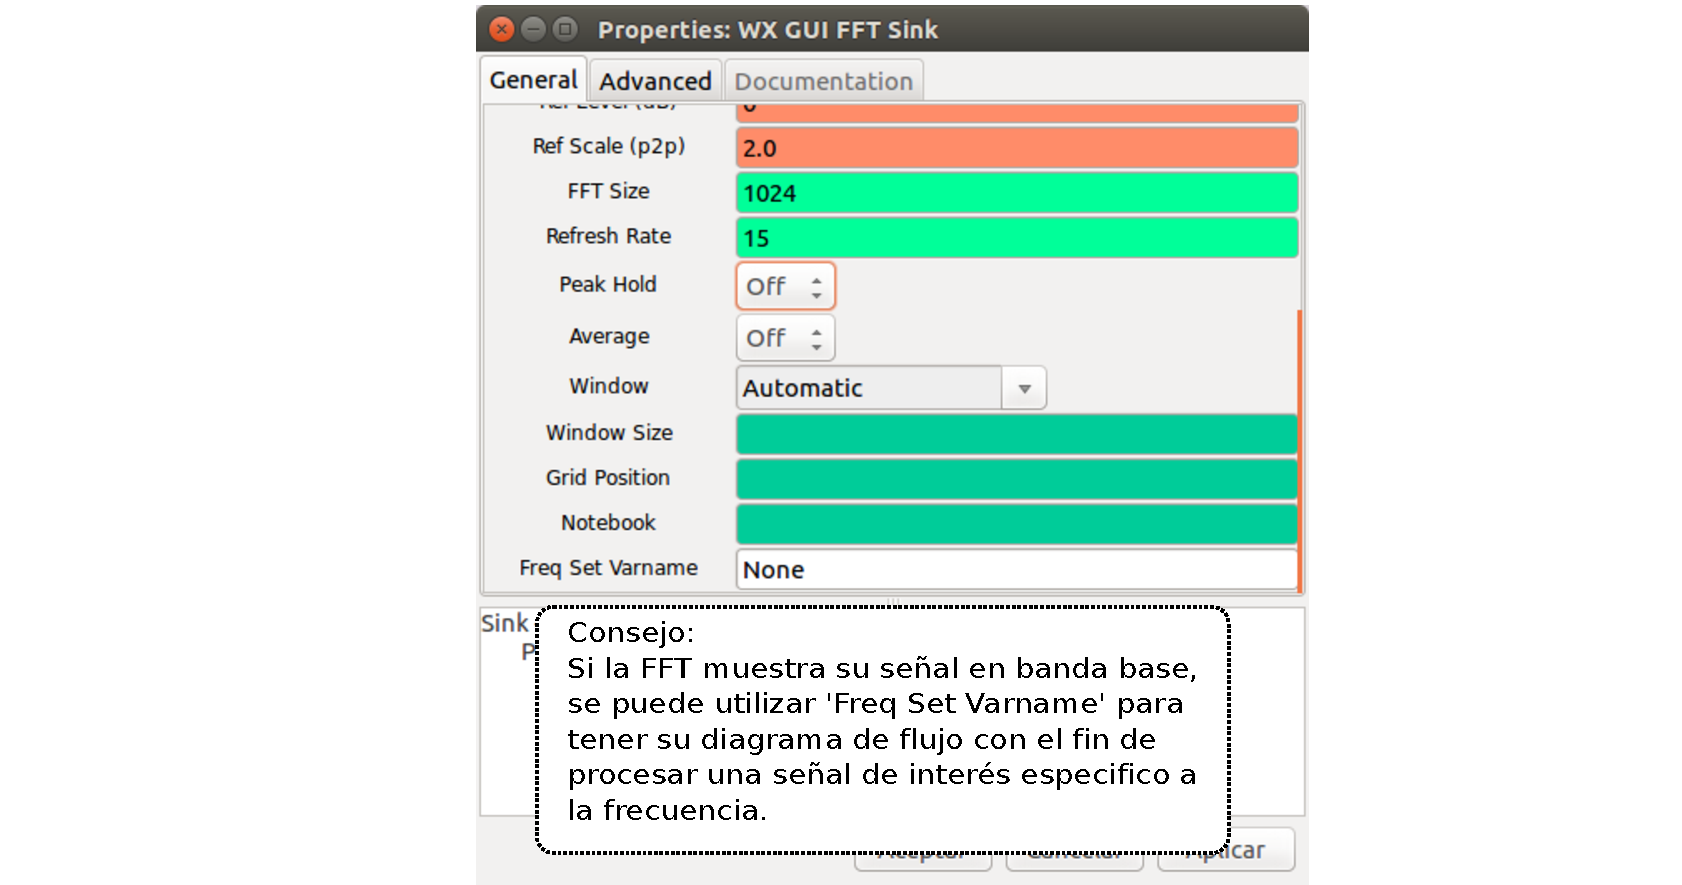
\includegraphics[width=1.1\textwidth]{parte1/lab2/pdf/lab2_8.pdf}
\end{figure}
\end{frame}
%--------------------------------

\begin{frame}{Osciloscopio y FFT\index{WX GUI FFT Sink}}
\begin{figure}[H]
\vspace{-3mm}
\centering
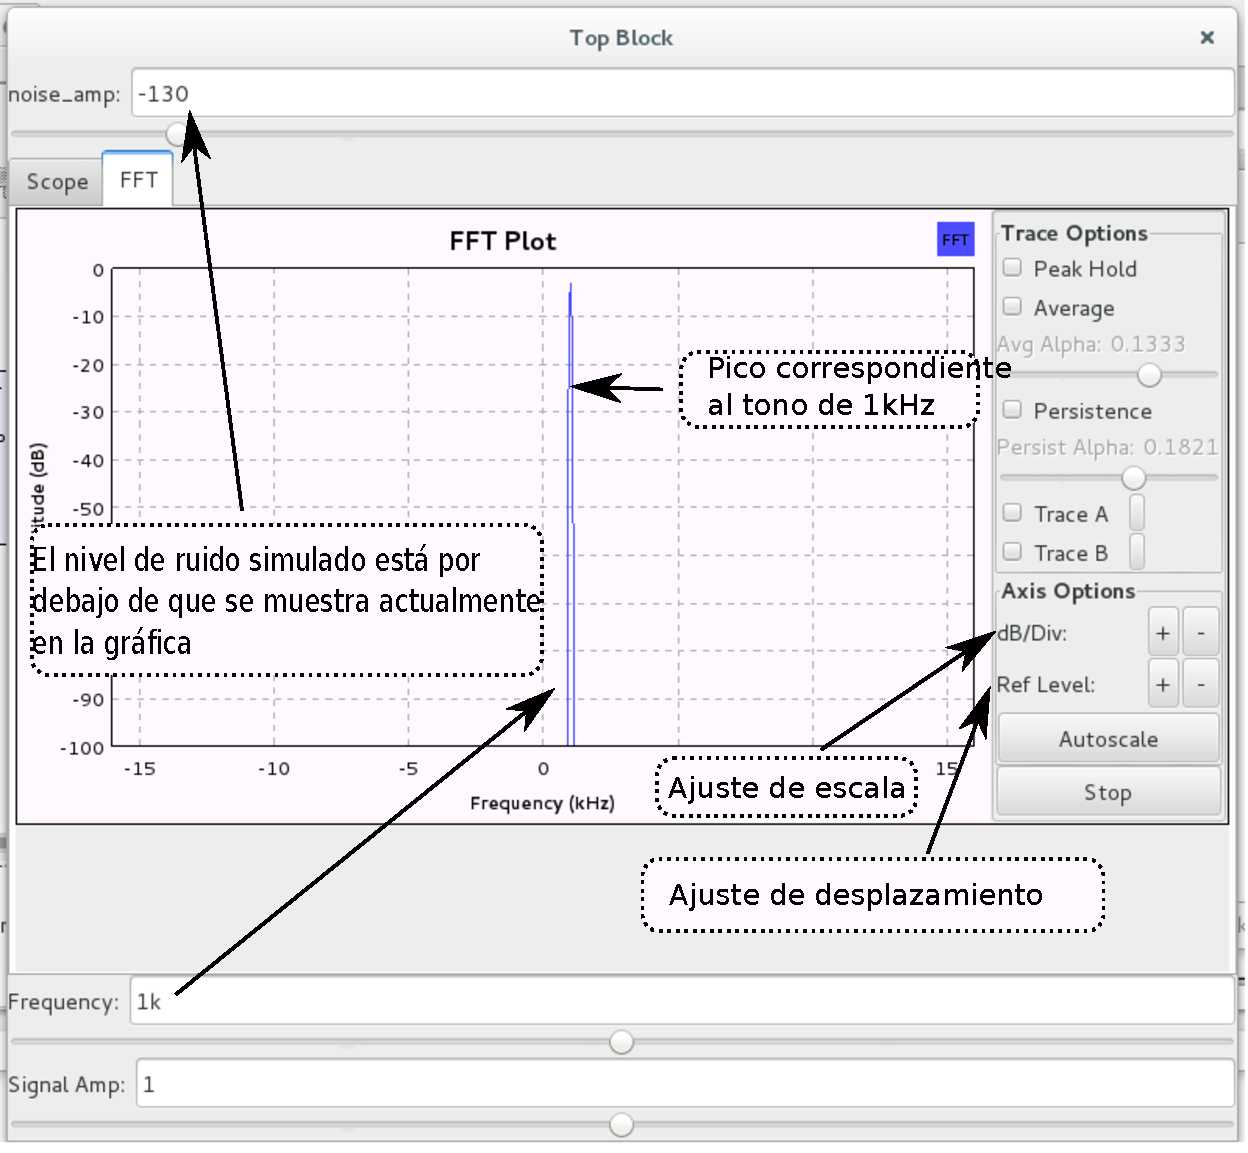
\includegraphics[width=0.7\textwidth]{parte1/lab2/pdf/lab2_9.pdf}
\end{figure}
\end{frame}
%--------------------------------

\begin{frame}{Osciloscopio y FFT}
\begin{figure}[H]
\vspace{-3mm}
\centering
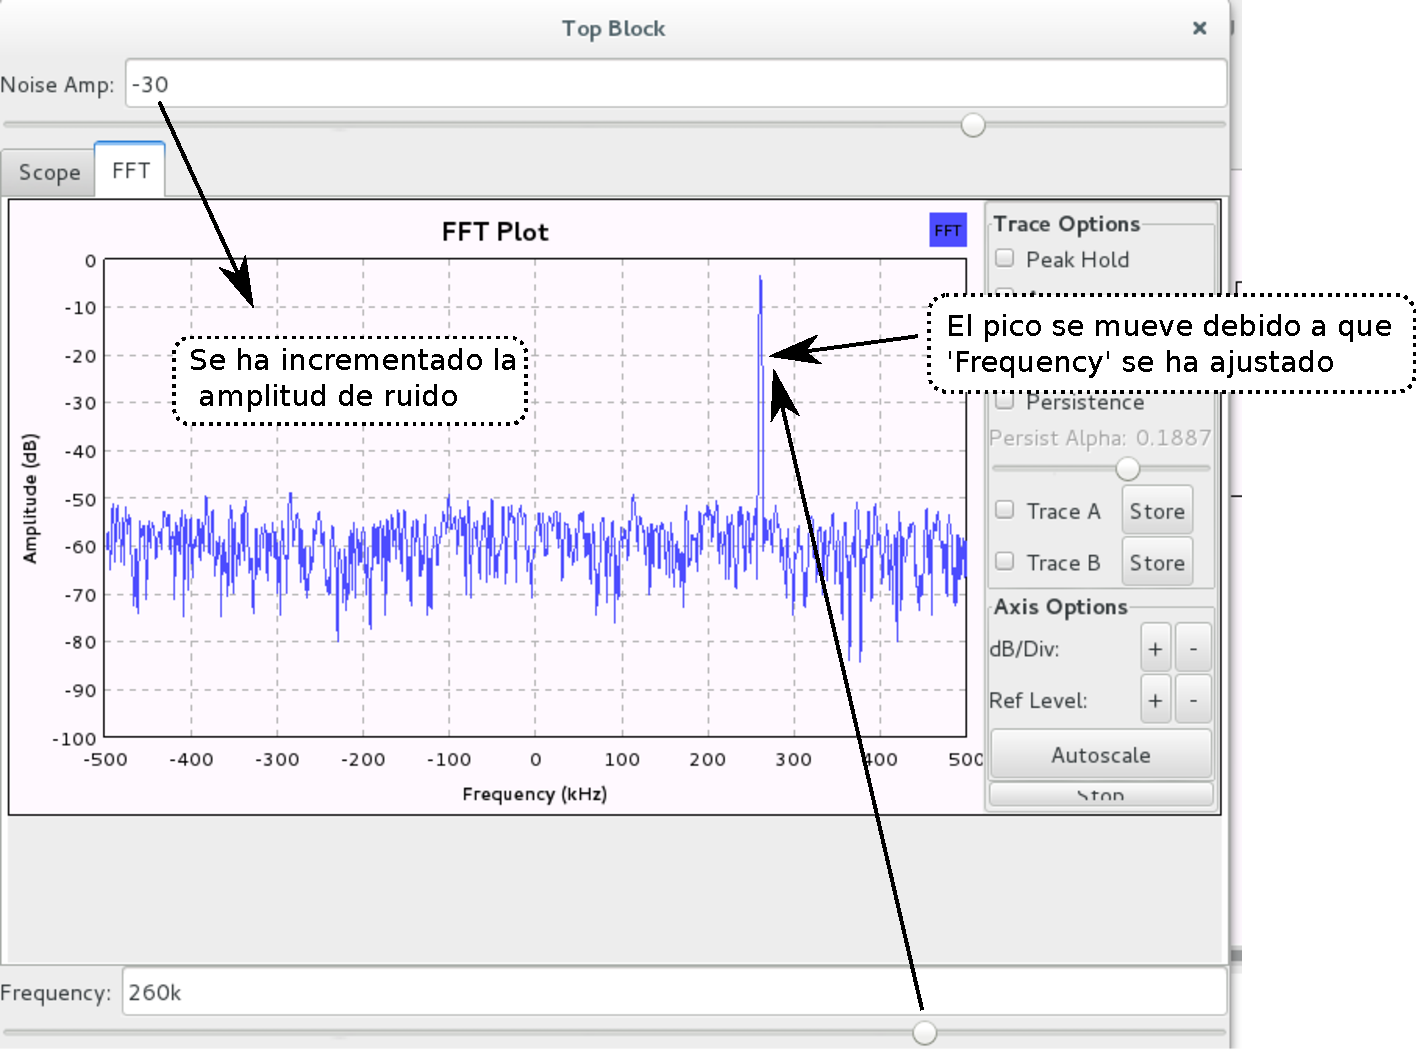
\includegraphics[width=0.85\textwidth]{parte1/lab2/pdf/lab2_10.pdf}
\end{figure}
\end{frame}
%--------------------------------

\begin{frame}{Osciloscopio y FFT}
\begin{figure}[H]
\vspace{-3mm}
\centering
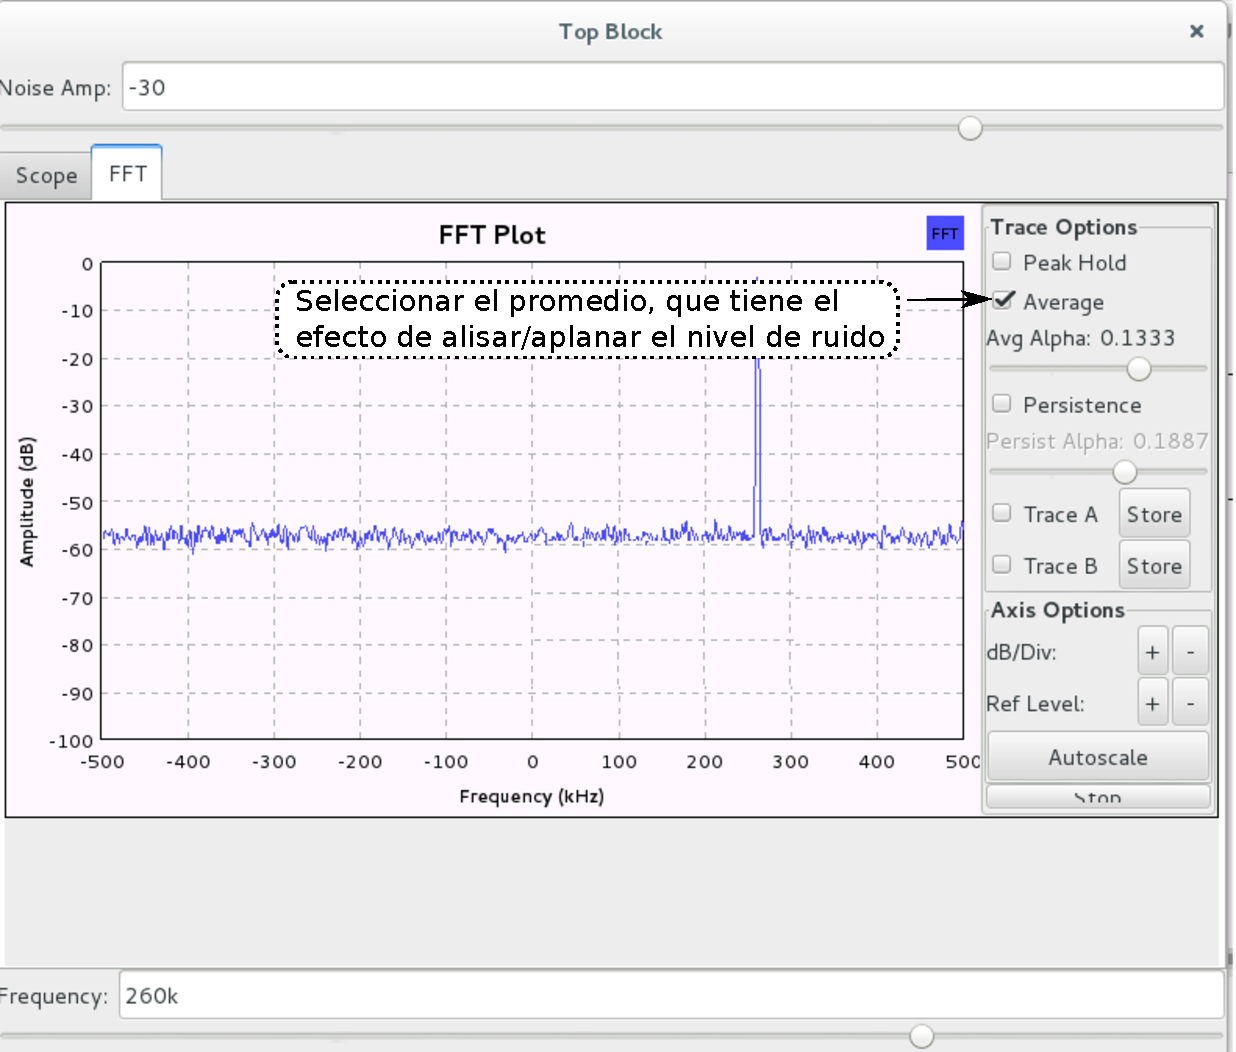
\includegraphics[width=0.75\textwidth]{parte1/lab2/pdf/lab2_11.pdf}
\end{figure}
\end{frame}
%--------------------------------

\begin{frame}{Osciloscopio y FFT}
\begin{figure}[H]
\vspace{-3mm}
\centering
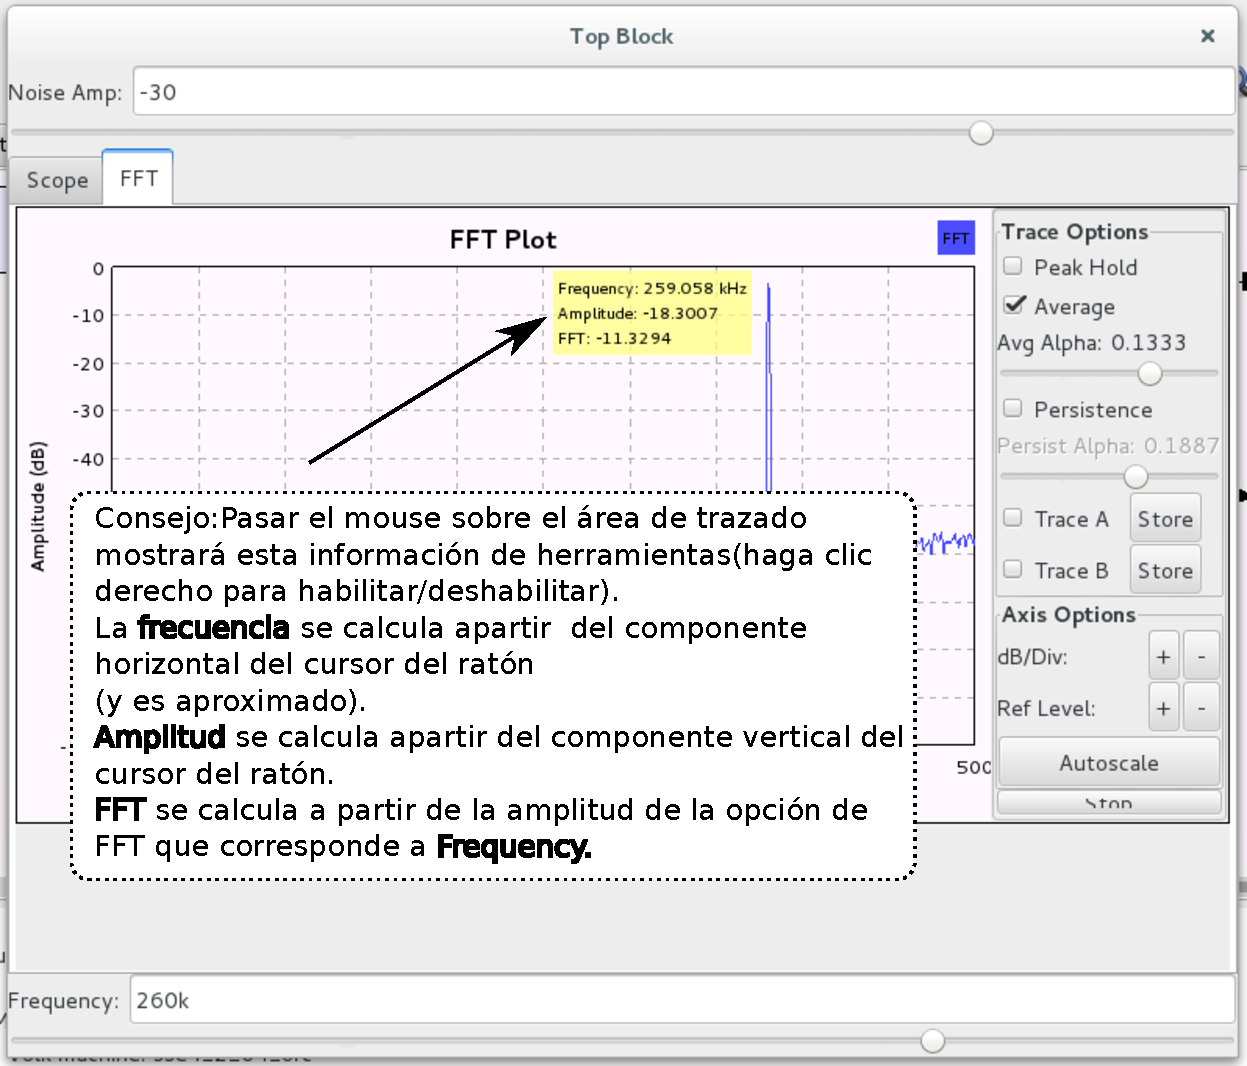
\includegraphics[width=0.75\textwidth]{parte1/lab2/pdf/lab2_12.pdf}
\end{figure}
\end{frame}
%--------------------------------

\begin{frame}{Osciloscopio y FFT}
\begin{figure}[H]
\centering
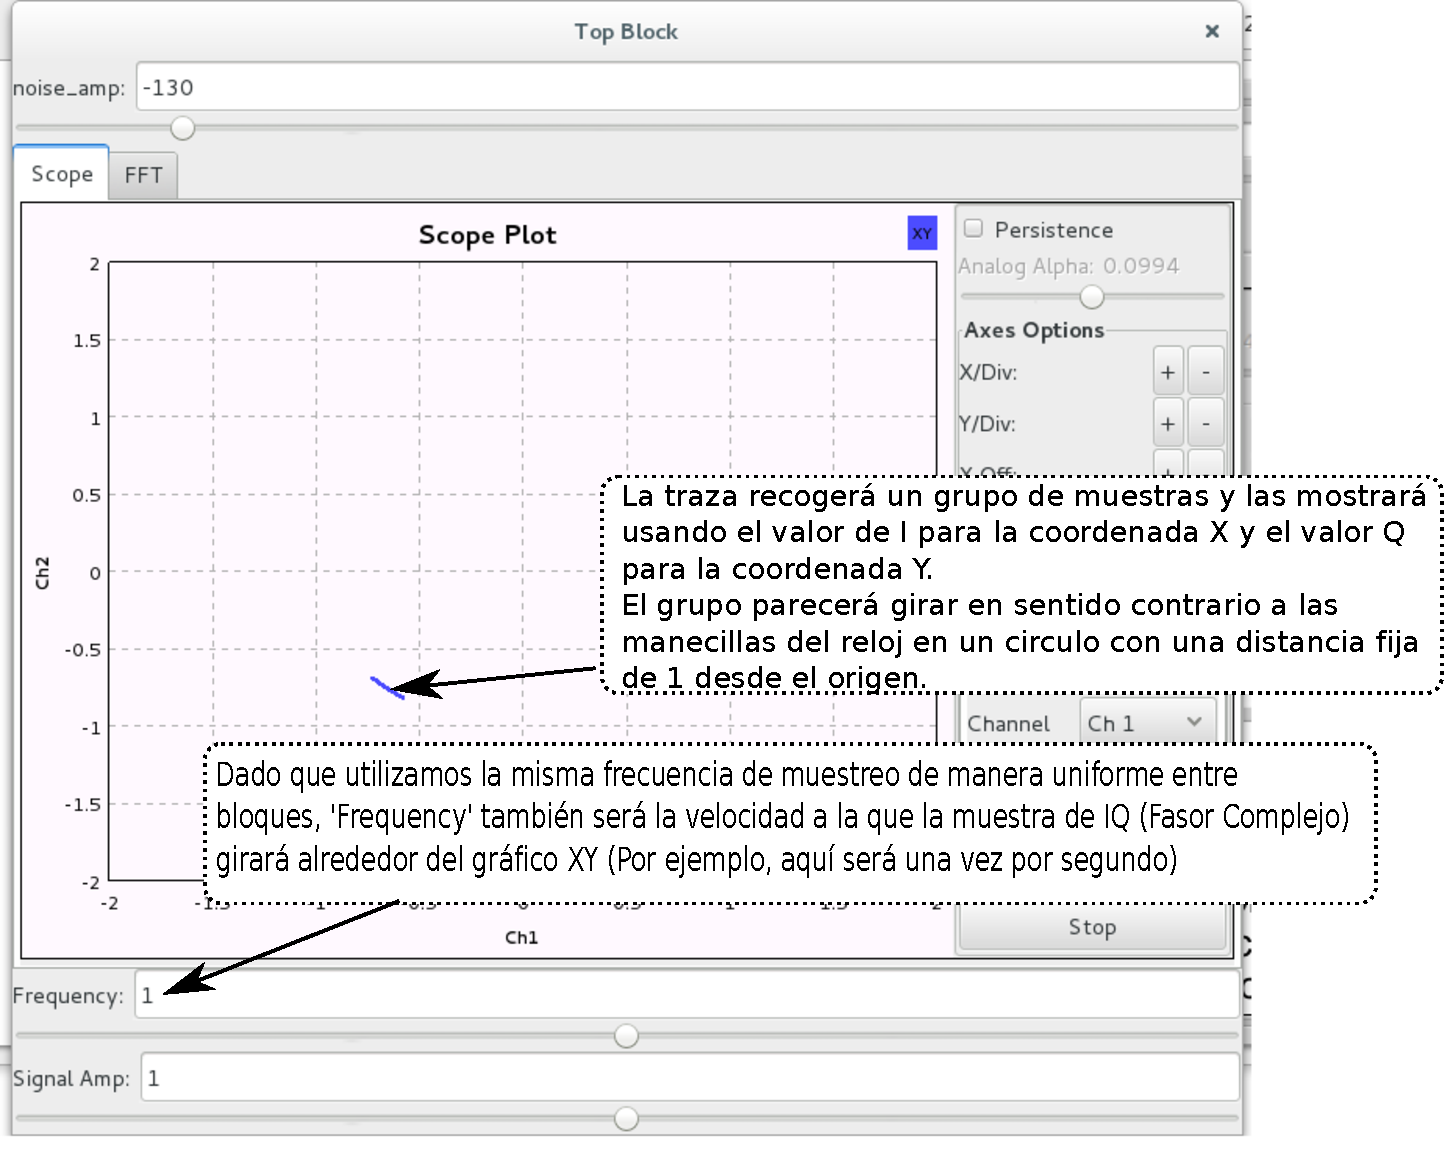
\includegraphics[width=0.75\textwidth]{parte1/lab2/pdf/lab2_13.pdf}
\end{figure}
\end{frame}
%--------------------------------

\begin{frame}{Osciloscopio y FFT}
\begin{figure}[H]
\vspace{-3mm}
\centering
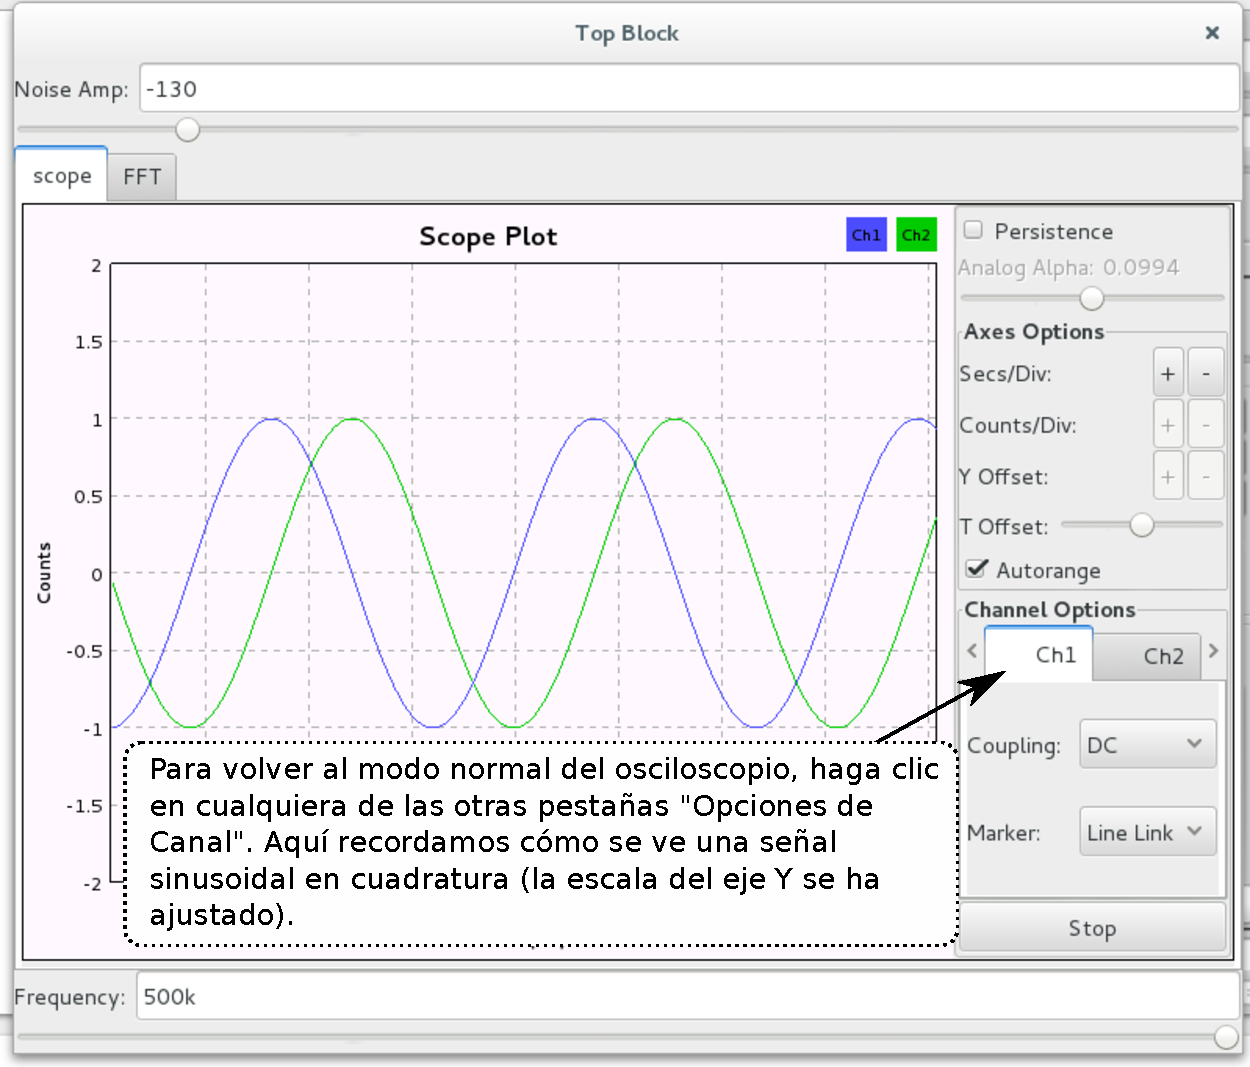
\includegraphics[width=0.75\textwidth]{parte1/lab2/pdf/lab2_14.pdf}
\end{figure}
\end{frame}
%--------------------------------

\begin{frame}{Osciloscopio y FFT}
\begin{figure}[H]
\vspace{-3mm}
\centering
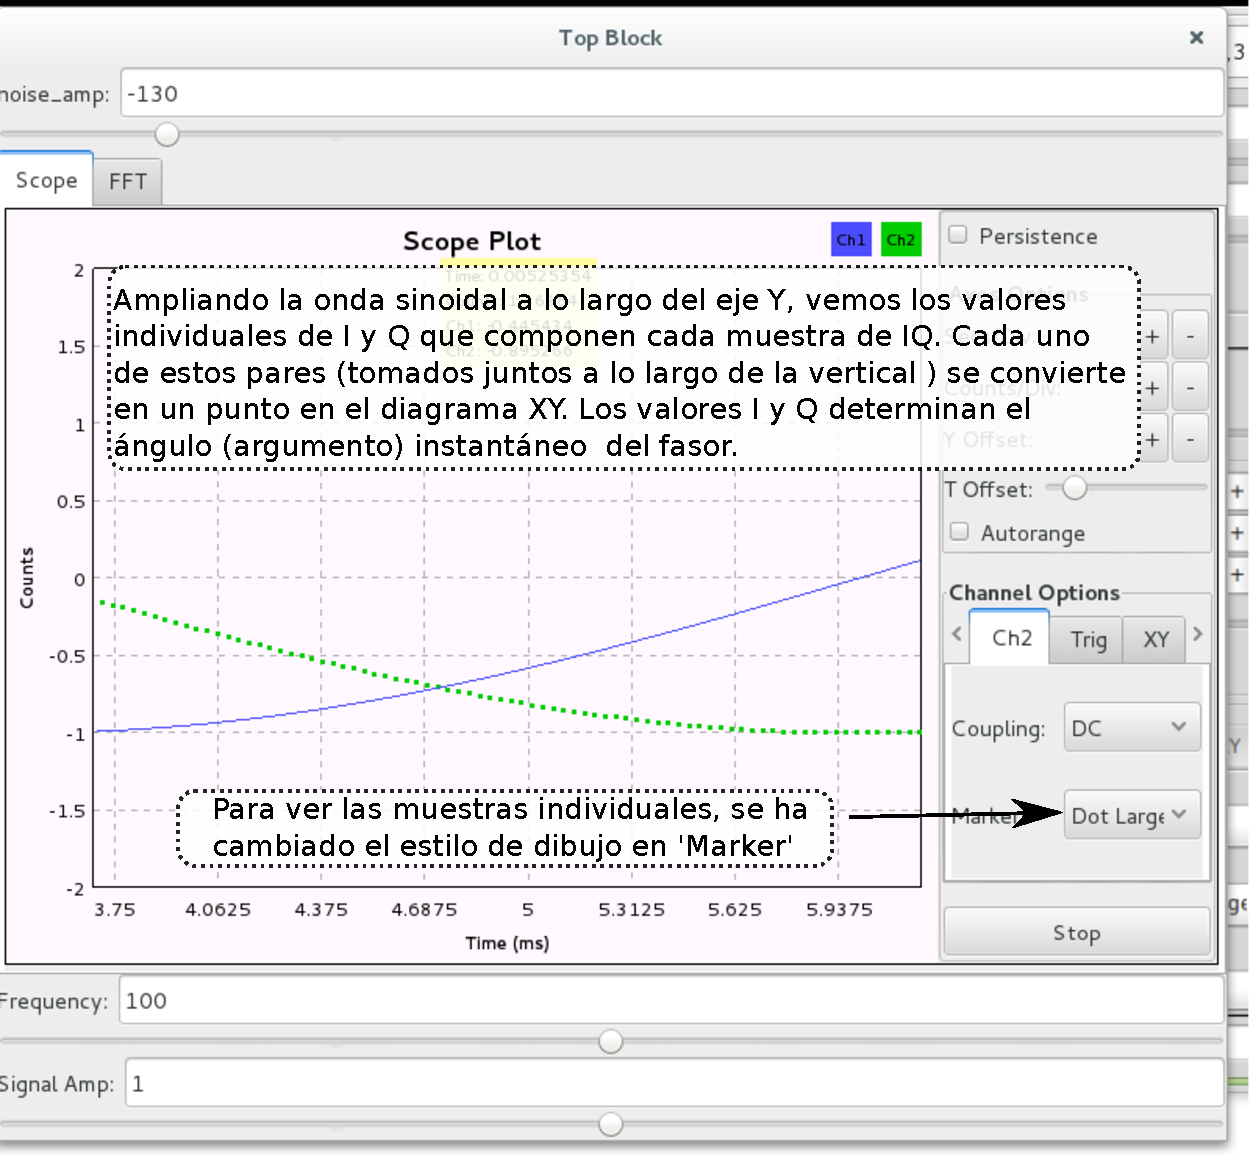
\includegraphics[width=0.7\textwidth]{parte1/lab2/pdf/lab2_15.pdf}
\end{figure}
\end{frame}
%--------------------------------

\begin{frame}{Osciloscopio y FFT}
\begin{figure}[H]
\centering
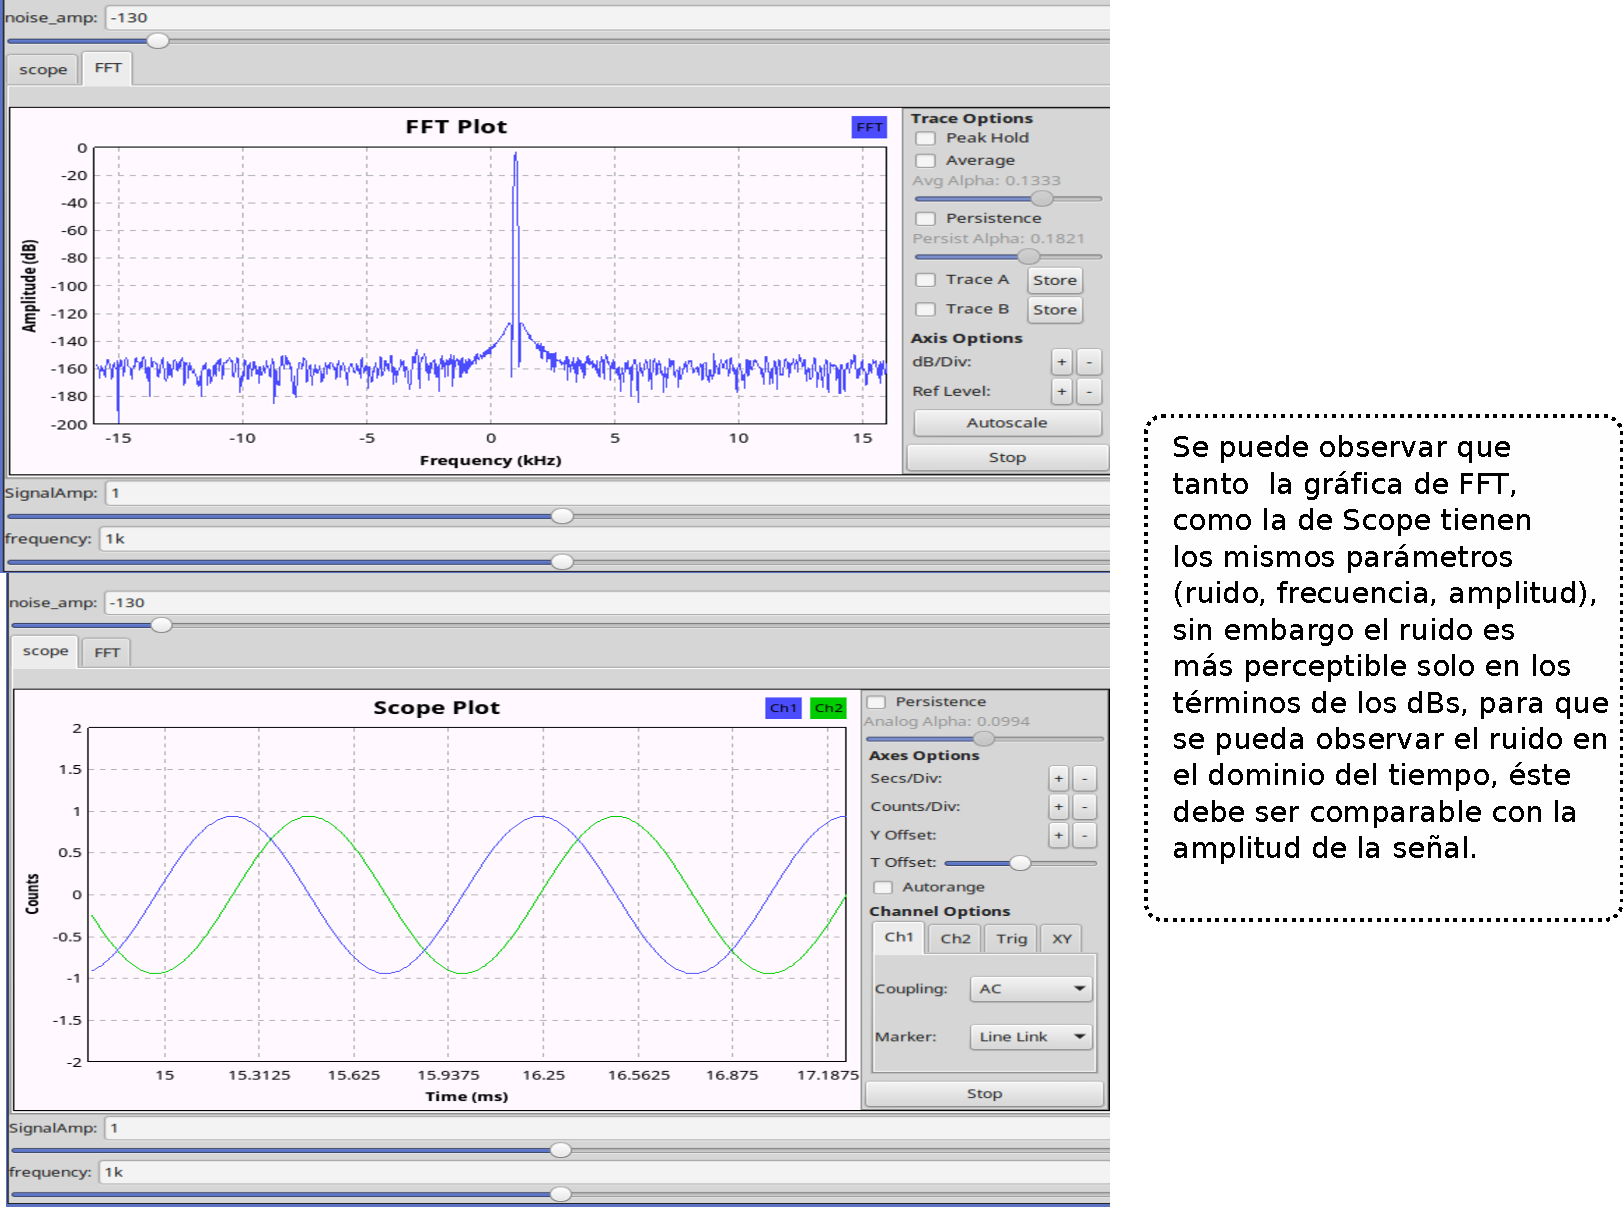
\includegraphics[width=\textwidth, height=0.58\textwidth]{parte1/lab2/pdf/lab2_16.pdf}
\end{figure}
\end{frame}
%--------------------------------